\documentclass[czech,12pt,a4paper,titlepage]{article}
\usepackage[left=15mm,right=15mm,top=25mm,bottom=25mm]{geometry}
\usepackage[autostyle]{csquotes}
\usepackage[export]{adjustbox}
\usepackage[czech]{babel}
\usepackage{graphicx}
\usepackage{utopia}

\title{%
    \textbf {MelodySphere} \\
    \bigskip
    \large Projekt do předmětu Databázové systémy I}
\author{Kateřina Baierová}
\date{}

\begin{document}

    \graphicspath{ {./img/} }

    \begin{titlepage}
        \maketitle
        \thispagestyle{empty}
    \end{titlepage}

    \tableofcontents

    \clearpage


    \section{Specifikace zadání}\label{sec:specifikace-zadani}
    \subsection*{Vize}
    Cílem webové aplikace je poskytovat uživatelům prostředí pro přehrávání hudby.
    Uživatel si vytvoří svůj osobní účet, který mu umožní nejen poslouchat
    hudbu svých oblíbených umělců, ale také vytvářet
    vlastní playlisty nebo hodnotit jednotlivé skladby.

    Dále poskytujeme možnost registrovat se jako umělec,
    což uživatelům umožňuje aktivně přispívat do hudební komunity.
    Umělci mohou přidávat vlastní skladby a vytvářet hudební alba.

    Aplikace má také uživatelům usnadňovat vyhledávání různých hudebních žánrů
    a poskytovat informace o jednotlivých umělcích.


    \subsection*{Role}
    \textbf{Uživatel} je osoba, která vytváří a spravuje svůj osobní účet.
    Po registraci získává možnost poslouchat hudbu, vytvářet vlastní playlisty
    a hodnotit jednotlivé skladby.
    Uživatelé mohou využívat funkce jako vyhledávání hudebních žánrů nebo
    získávat informace o umělcích.
    \textbf{Umělec} je uživatel s registrovaným účtem, který má zájem aktivně přispívat do hudební komunity.
    Může přidávat vlastní skladby a vytvářet hudební alba, která jsou dostupná pro poslech ostatním uživatelům.
    Umělci mají možnost prezentovat svou tvorbu a budovat svůj profil.

    \subsection*{Vstupy}
    text

    \subsection*{Výstupy}
    text

    \subsection*{Funkce}
    text

    \clearpage


    \section{Datová analýza}\label{sec:datova-analyza}
    \subsection*{Konceptuální datový model}
    graf
    %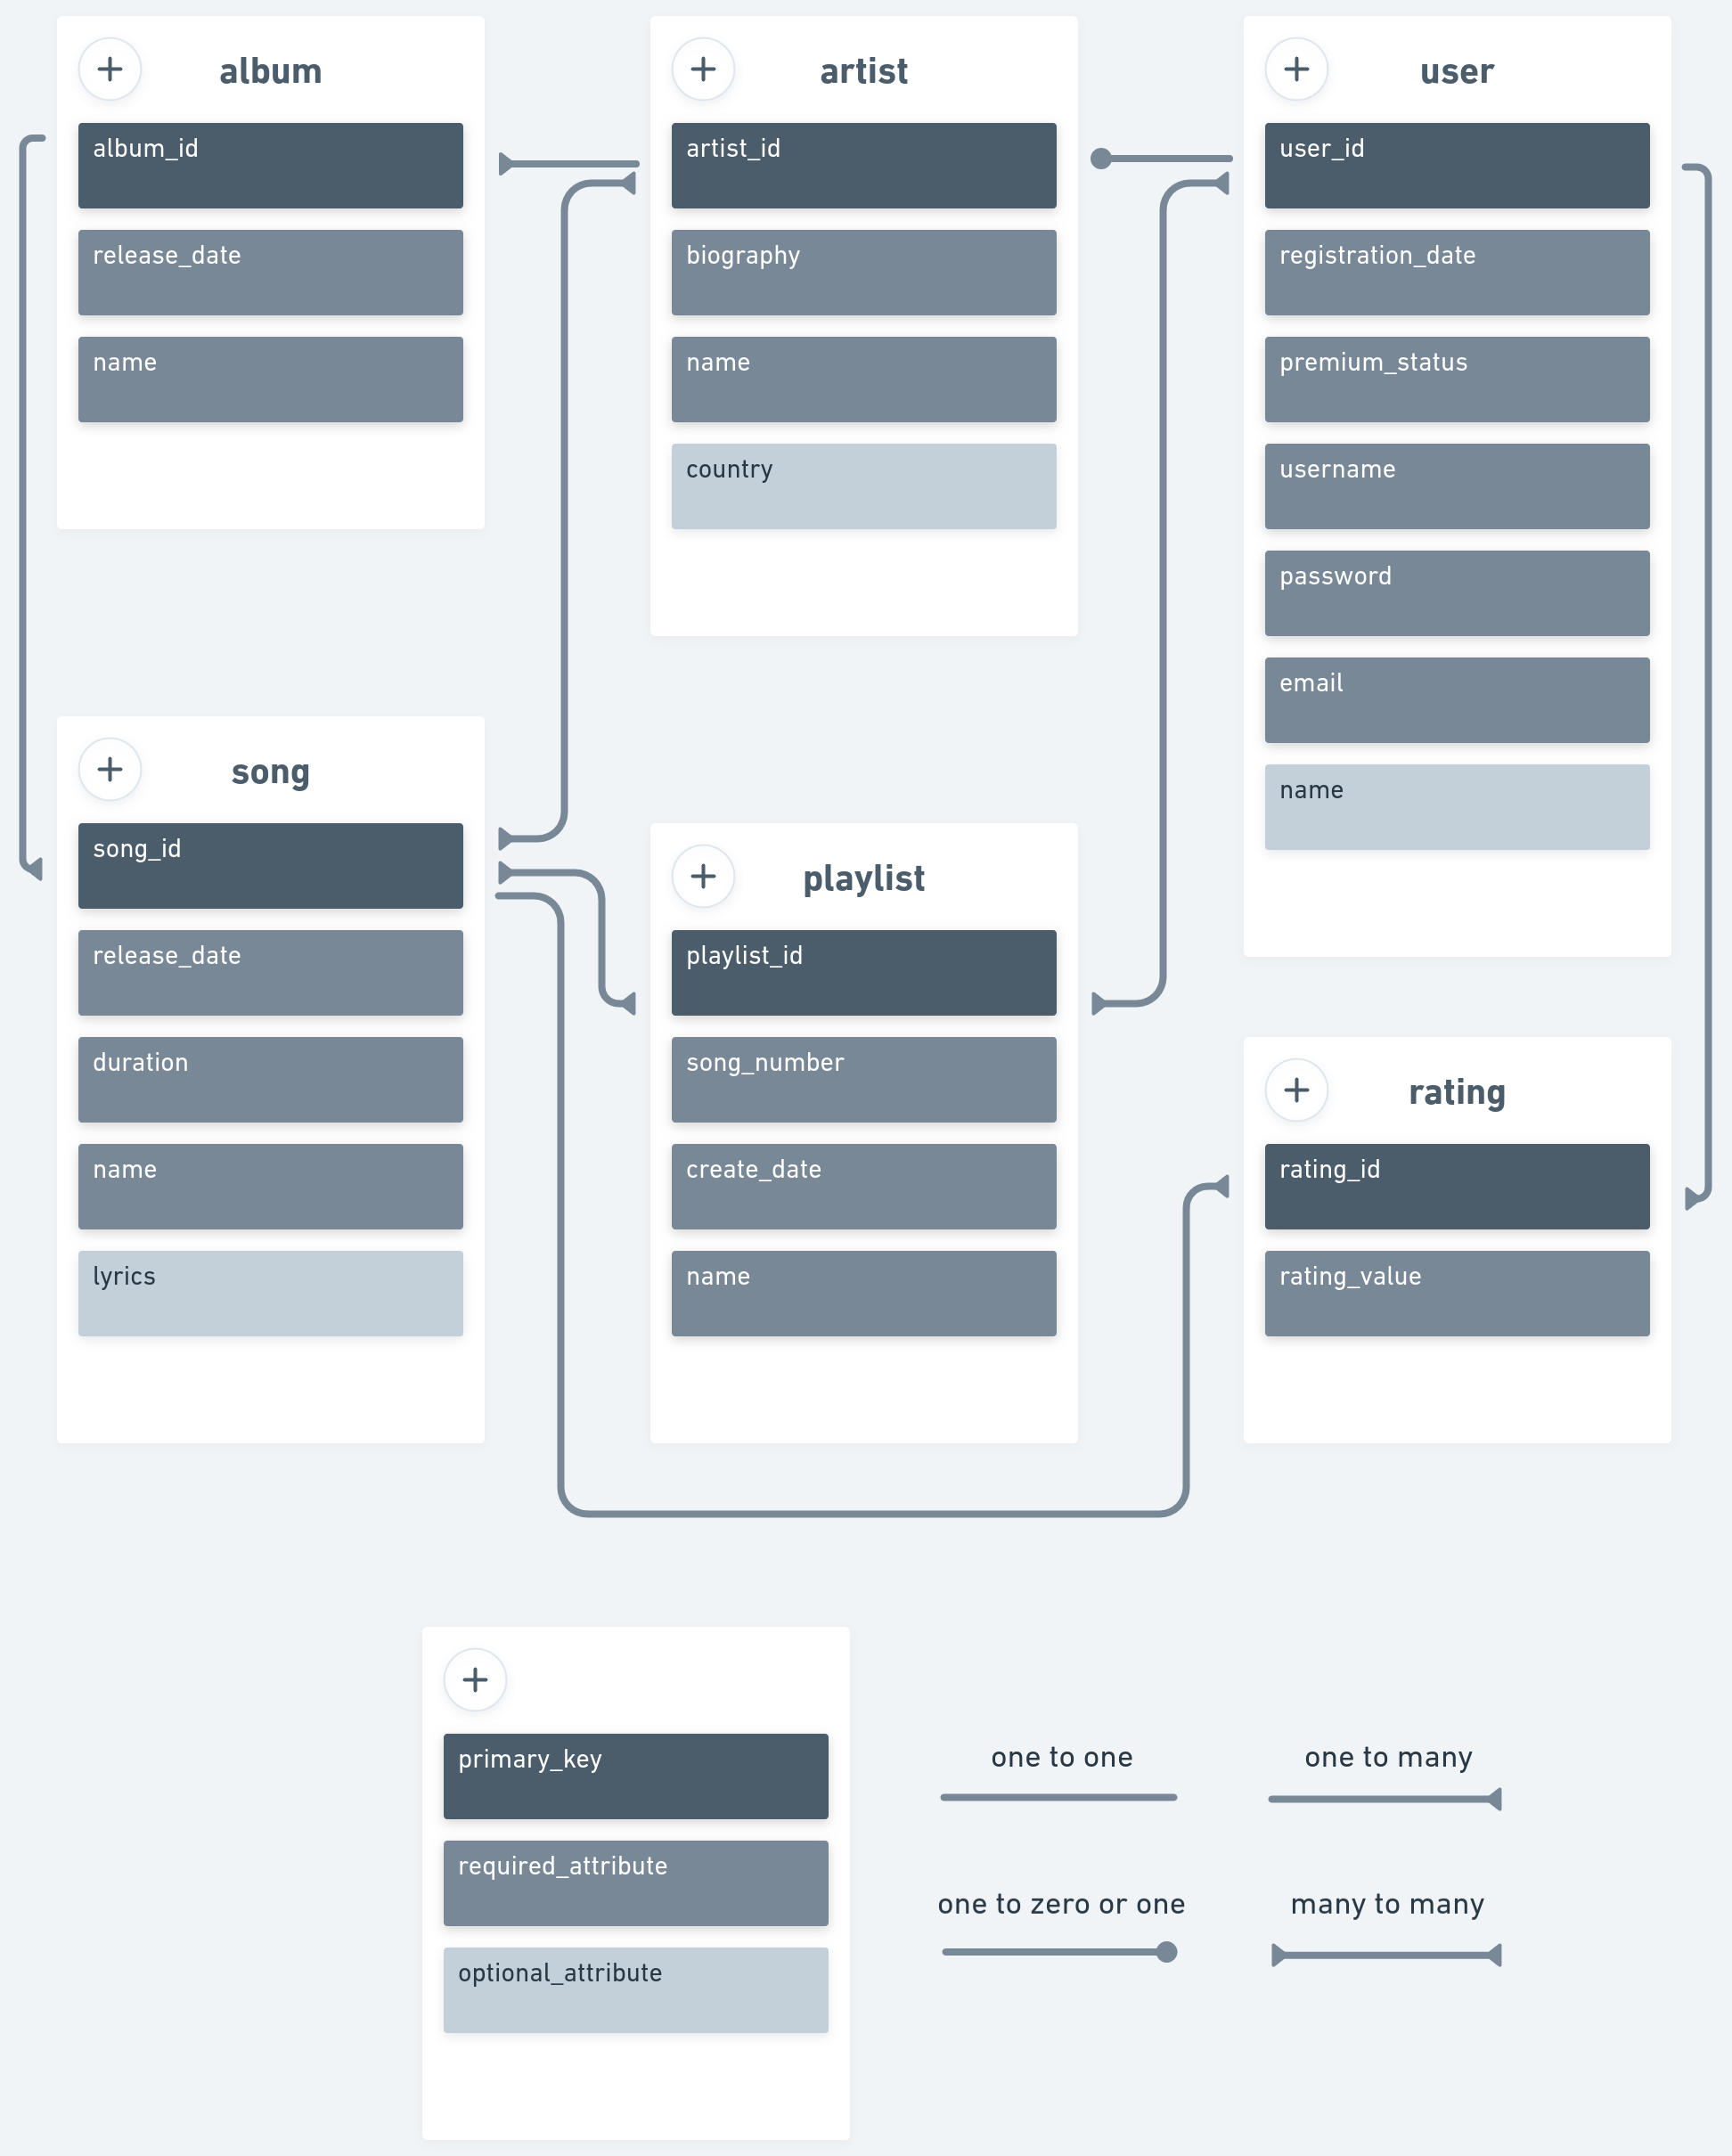
\includegraphics[width=0.9 \textwidth, center]{konceptualni_datovy_model}

    \subsection*{Relační datový model}
    \bigskip
    \bigskip
    \bigskip
    graf
    %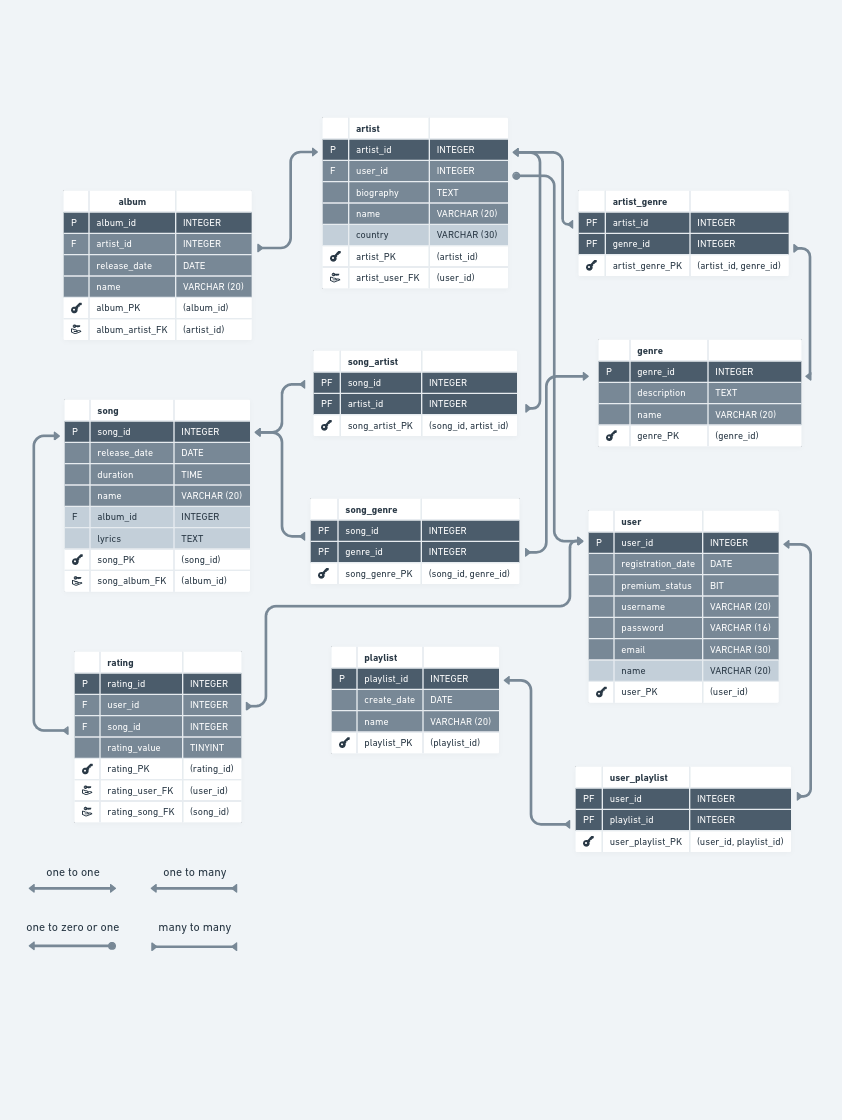
\includegraphics[width=1\textwidth, center]{relacni_datovy_model}

    \clearpage

    \section*{Datový slovník}
    Popis jednotlivých tabulek je uveden v následujícím datovém slovníku.

\subsection*{User}
\begin{tabular}{ |c|c c c c c|c| }
    \hline
    \textbf{Název atributu} & \textbf{Datový typ} & \textbf{Délka} & \textbf{Klíč} & \textbf{Null} & \textbf{IO} & \textbf{Popis}                         \\
    \hline
    user\_id                & INTEGER             &                & Primární      & Ne            &             & Automaticky inkrementovaný PK   \\
    registration\_date      & DATE                &                &               & Ne            &             & Datum registrace uživatele      \\
    premium\_status         & BIT                 &                &               & Ne            &             & Status prémiového účtu          \\
    username                & VARCHAR             & 20             &               & Ne            &             & Přezdívka uživatele             \\
    password                & VARCHAR             & 16             &               & Ne            & 3           & Heslo uživatele                 \\
    email                   & VARCHAR             & 30             &               & Ne            &             & E-mail uživatele pro přihlášení \\
    name                    & VARCHAR             & 20             &               & Ano           &             & Jméno uživatele                 \\
    \hline
\end{tabular}
\bigskip

\subsection*{Song}
\begin{tabular}{ |c|c c c c c|c| }
    \hline
    \textbf{Název atributu} & \textbf{Datový typ} & \textbf{Délka} & \textbf{Klíč} & \textbf{Null} & \textbf{IO} & \textbf{Popis}                         \\
    \hline
    song\_id                & INTEGER             &                & Primární      & Ne            &             & Automaticky inkrementovaný PK   \\
    release\_date           & DATE                &                &               & Ne            &             & Datum vydání skladby            \\
    duration                & TIME                &                &               & Ne            & 1           & Délka skladby                   \\
    name                    & VARCHAR             & 20             &               & Ne            &             & Název skladby                   \\
    album\_id               & INTEGER             &                & Cizí (Album)  & Ano           &             & Album, do kterého skladba patří \\
    lyrics                  & TEXT                &                &               & Ano           &             & Text ke skladbě                 \\
    \hline
\end{tabular}
\bigskip

\subsection*{Artist}
\begin{tabular}{ |c|c c c c c|c| }
    \hline
    \textbf{Název atributu} & \textbf{Datový typ} & \textbf{Délka} & \textbf{Klíč} & \textbf{Null} & \textbf{IO} & \textbf{Popis}                         \\
    \hline
    artist\_id              & INTEGER             &                & Primární      & Ne            &             & Automaticky inkrementovaný PK \\
    user\_id                & INTEGER             &                & Cizí (User)   & Ne            &             & Správce účtu                  \\
    biography               & TEXT                &                &               & Ne            &             & Biografie tvůrce              \\
    name                    & VARCHAR             & 20             &               & Ne            &             & Jméno tvůrce                  \\
    country                 & VARCHAR             & 30             &               & Ano           &             & Země původu                   \\
    \hline
\end{tabular}
\bigskip

\subsection*{Album}
\begin{tabular}{ |c|c c c c c|c| }
    \hline
    \textbf{Název atributu} & \textbf{Datový typ} & \textbf{Délka} & \textbf{Klíč} & \textbf{Null} & \textbf{IO} & \textbf{Popis}                         \\
    \hline
    album\_id               & INTEGER             &                & Primární      & Ne            &             & Automaticky inkrementovaný PK \\
    artist\_id              & INTEGER             &                & Cizí (Artist) & Ne            &             & Tvůrce alba                   \\
    release\_date           & DATE                &                &               & Ne            &             & Datum vydání alba             \\
    name                    & VARCHAR             & 20             &               & Ne            &             & Jméno alba                    \\
    \hline
\end{tabular}
\bigskip

\subsection*{Rating}
\begin{tabular}{ |c|c c c c c|c| }
    \hline
    \textbf{Název atributu} & \textbf{Datový typ} & \textbf{Délka} & \textbf{Klíč} & \textbf{Null} & \textbf{IO} & \textbf{Popis}                         \\
    \hline
    rating\_id              & INTEGER             &                & Primární      & Ne            &             & Automaticky inkrementovaný PK \\
    user\_id                & INTEGER             &                & Cizí (User)   & Ne            &             & Hodnotící uživatel            \\
    song\_id                & INTEGER             &                & Cizí (Song)   & Ne            &             & Hodnocená skladba             \\
    rating\_value           & TINYINT             &                &               & Ne            & 2           & Samotné ohodnocení            \\
    \hline
\end{tabular}
\bigskip

\subsection*{Playlist}
\begin{tabular}{ |c|c c c c c|c| }
    \hline
    \textbf{Název atributu} & \textbf{Datový typ} & \textbf{Délka} & \textbf{Klíč} & \textbf{Null} & \textbf{IO} & \textbf{Popis}                         \\
    \hline
    playlist\_id            & INTEGER             &                & Primární      & Ne            &             & Automaticky inkrementovaný PK \\
    create\_date            & DATE                &                &               & Ne            &             & Datum vytvoření playlistu     \\
    name                    & VARCHAR             & 20             &               & Ne            &             & Název playlistu               \\
    \hline
\end{tabular}
\bigskip

\subsection*{Song\_artist}
\begin{tabular}{ |c|c c c c c|c| }
    \hline
    \textbf{Název atributu} & \textbf{Datový typ} & \textbf{Délka} & \textbf{Klíč} & \textbf{Null} & \textbf{IO} & \textbf{Popis}                         \\
    \hline
    song\_id                & INTEGER             &                & Cizí (Song)   & Ne            &             & Vytvořená skladba \\
    artist\_id              & INTEGER             &                & Cizí (Artist) & Ne            &             & Tvůrce skladby    \\
    \hline
\end{tabular}
\bigskip

\subsection*{Song\_playlist}
\begin{tabular}{ |c|c c c c c|c| }
    \hline
    \textbf{Název atributu} & \textbf{Datový typ} & \textbf{Délka} & \textbf{Klíč}   & \textbf{Null} & \textbf{IO} & \textbf{Popis}                         \\
    \hline
    song\_id                & INTEGER             &                & Cizí (Song)     & Ne            &             & Daná skladba   \\
    playlist\_id            & INTEGER             &                & Cizí (Playlist) & Ne            &             & Dany laylist   \\
    \hline
\end{tabular}
\bigskip

\subsection*{User\_playlist}
\begin{tabular}{ |c|c c c c c|c| }
    \hline
    \textbf{Název atributu} & \textbf{Datový typ} & \textbf{Délka} & \textbf{Klíč}   & \textbf{Null} & \textbf{IO} & \textbf{Popis}                         \\
    \hline
    user\_id                & INTEGER             &                & Cizí (USer)     & Ne            &             & Tvůrce playlistu   \\
    playlist\_id            & INTEGER             &                & Cizí (Playlist) & Ne            &             & Vytvořený playlist \\
    \hline
\end{tabular}
\bigskip

\subsubsection*{Integritní omezení:}
\begin{enumerate}
    \item \textit{duration} musí mít maximálně 15 minut.
    \item \textit{rating\_value} může nabýt pouze hodnoty 1--5.
    \item \textit{password} musí obsahovat minimálně 6 znaků.
\end{enumerate}

\end{document}
